
\chapter{Space-time coupling} \label{ssn_time_dependent_problems}

\begin{figure}
  \centering
    %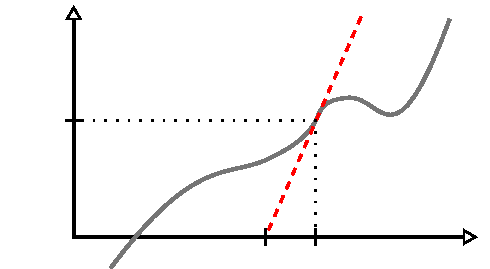
\includegraphics[width=\linewidth]{images/newton_raphson.pdf}
    \def\svgwidth{\linewidth}
    \input{images/fenics_intro/svg/alpha_approximation.pdf_tex}
  \caption[$\alpha$-family of time derivative approximation]{Oh yeah!}
  \label{alpha_family_image}
\end{figure}

For a function $u = u(x,t)$, the time derivative of $u$ at any given time $t+\alpha \Delta t$ can be stated as a linear interpolation of the time derivative between times $t$ and $t + \Delta t$.  That is,
\begin{align}
  \label{alpha_family_derivative}
  \dot{u}_{t + \alpha \Delta t} = \alpha \dot{u}_{t + \Delta t} + (1-\alpha) \dot{u}_t,
\end{align}
where $\alpha \in [0,1]$.  First, assume that we have already determined the value of $u$ at time step $t$, and that we would like to determine $u$ for the next time step $t + \Delta t$.  For some intermediate timestep $t + \alpha \Delta t$, the time derivative of $u$ may be estimated using mean value theorem definition (\ref{mean_value_theorem}) \index{Mean value theorem!discrete time derivative} as
\begin{align*}
  \totder{}{t} u(x,t + \alpha \Delta t) = \frac{u_{t + \Delta t} - u_t}{\Delta t} \hspace{10mm} \text{for some $\alpha \in [0,1]$},
\end{align*}
which when combined with linear interpolation (\ref{alpha_family_derivative}) yields \index{Time derivatives!$\alpha$-family approximation}
\begin{align}
  \label{generalized_time_derivative}
  \frac{u_{t + \Delta t} - u_t}{\Delta t} = \alpha \dot{u}_{t + \Delta t} + (1-\alpha) \dot{u}_t.
\end{align}

As illustrated in Figure \ref{alpha_family_image}, the difficulty with this equation resides in finding an appropriate value for $\alpha$.  Recall that the objective is to determine the value of $u$ at time step $t+\Delta t$.  A natural first choice is to make $\alpha = 1$ so that we can solve for $u = u(x,t+\Delta t)$ directly.  In this case, relation (\ref{generalized_time_derivative}) provides \index{Time derivatives!Forward difference}
\begin{align}
  \label{forward_difference}
  \totder{}{t} u(x,t+\Delta t) = \frac{u_{t+\Delta t} - u_t}{\Delta t} \hspace{5mm} \leftarrow \text{forward difference}.
\end{align}
Likewise, taking $\alpha = 0$ allows us to solve for the time derivative of the current value $u = u(x,t)$ \index{Time derivatives!Backward difference}
\begin{align}
  \label{backward_difference}
  \phantom{tt + \Delta t} \totder{}{t} u(x,t) = \frac{u_{t + \Delta t} - u_t}{\Delta t} \hspace{5mm} \leftarrow \text{backward difference}.
\end{align}
The designation as \emph{forward-} or \emph{backward-difference} references the evaluation position in time of the time derivative of the function $u(x,t)$; either at the next or previous time step, respectively.

The specific choice of $\alpha$ will make a large difference on the quality of the approximation as time increases.  First, note that stating the time derivative of $u$ as forward difference relation (\ref{forward_difference}) solves for the value of the function $u(x,t)$ at the next time step \emph{explicitly}.  That is, in this case the time derivative $\dot{u}$ is unknown and determined in the process of solving for $u$.  Similarly, backward-difference formulation (\ref{backward_difference}) solves for the subsequent value of $u(x, t)$ \emph{implicitly}, in the sense that the time derivative $\dot{u}$ has been determined from the previous time-step and used directly to calculate the next value of $u$.

Constraining the time-derivative of backward-difference formulation (\ref{backward_difference}) to be a function of the previous time-step exclusively has the effect of making this equation stable.  For the same reasoning, forward-difference formulation (\ref{forward_difference}) is only stable under certain conditions.

There are many other intermediate values that may be chosen for $\alpha$, which are referred to as \emph{semi-implicit}.  Popular $\alpha$-values are summaraized below.
\begin{align*}
    \alpha = 
    \begin{cases}
      1,                   & \text{backward-Euler (implicit)}\\
      \nicefrac{2}{3},     & \text{Galerkin}\\
      0.878,               & \text{Liniger}\\
      \nicefrac{1}{2},     & \text{Crank-Nicolson}\\
      0,                   & \text{forward-Euler (explicit)}
    \end{cases}
\end{align*}
The Liniger value of $\alpha = 0.878$ was derived by \citet{liniger_1968} as the solution to the optimization problem
\begin{align*}
  \min_{\alpha} \left\{ \hspace{2mm} \max_{0 \leq \tau \leq \infty} \left| \exp(-\tau) - \frac{1 - (1-\alpha)\tau}{1 + \alpha \tau} \right| \hspace{2mm} \right\}.
\end{align*}
